% Chapter 17: One Oscillator Vibrates; Many Make a Wave
\chapter{One Oscillator Vibrates; Many Make a Wave}

\step{A Counterintuitive Opening}

\begin{mainline}
During PE, you call to Xiaoming a hundred meters across the field. About a third of a second later, he turns around.

Think carefully: how did your voice get there?

The easy answer is that air carried it. But if air really left your mouth and raced toward Xiaoming at 340 meters per second, it would be a gale strong enough to ruffle his hair and overturn his notebook. Nothing of the kind happens. His surrounding air stays near him, and yours stays near you.

Nothing traveled across, yet something arrived.

Other puzzles share this form. Slap one end of a swimming pool and a plastic duck at the other end bobs, barely drifting toward or away from you. Tens of thousands of spectators make a stadium wave that circles the stands in seconds, yet everyone remains at their own seat. The wave arrives, but nobody takes a step.

This chapter asks what that something is: it arrives even though no object travels across.
\end{mainline}

\step{Make a Guess First}

\begin{mainline}
Before continuing, place a bet. Picture a long rope tied to a door handle, with its other end in your hand. Flick your wrist up and down and a bump runs toward the handle.

Give your intuitive judgment on three questions:

\begin{itemize}
  \item How fast does the bump travel? Does it depend on how hard you flick or how tightly the rope is stretched?
  \item What happens at the handle: does the bump disappear, stop, or turn back?
  \item If two people holding opposite ends flick simultaneously, do the approaching bumps collide and bounce apart like balls?
\end{itemize}

Record your answers for checking later. One spoiler: most people miss the third, for the most useful reason. It forces a clean separation between waves and flying objects.
\end{mainline}

\step{Hands-on Experiment}

\begin{experiment}[Waves on a Rope]
You need a three-to-five-meter rope, such as a skipping rope, clothesline, or backpack strap, a partner, and a phone.

First, observe qualitatively. Tie one end to a table leg and hold the other, just lifting the slightly taut rope off the ground. Flick upward and return your wrist. A bump runs out, reaches the leg, and, watch carefully, turns back. That is our second prediction question.

Second, make the bump stand still. Tighten the rope and move your wrist continuously side to side or up and down at a steady beat. Adjust the rhythm until the rope stops moving chaotically and takes a stable shape, largest in the middle, like a frozen wave. Faster rhythms produce two or three sections moving oppositely. Remember that the shape steadies only at the right rhythm. Later we call it a standing wave.

Third, measure. Have your partner sharply pull one end to make a bump while you time its end-to-end travel with a phone stopwatch. Average three trials. Measure rope length with a tape; speed equals length divided by time. Tighten the rope and repeat. The same rope carries bumps faster when tighter. Wave speed depends on the rope's state, not your flick's strength. Our mathematical translator will make this a formula.

Safety: do not use a highly elastic rubber cord; if released under tension, it can lash someone.
\end{experiment}

\step{The Old Model Runs into Trouble}

\begin{mainline}
So far, our approach has been to identify objects, record their positions, velocities, and forces, and use Newton's laws to predict what follows. Springs and pendulums fit. What happens when we apply it to a traveling rope bump?

First difficulty: too many objects. No little piece of rope relocates to the table leg. After the bump passes, every segment remains near its original position, having moved only up and down. The bump is not a moving object. What is it, then? We cannot draw a free-body diagram for nothing. Water waves make the discomfort clearer: a floating leaf rises and falls locally while the crest advances many meters. Insisting that motion needs a traveling object seems to require an invisible object crossing the pond.

Second: divide the rope into a hundred little oscillators and track each, and another question appears. Why must each follow its neighbor? Your hand never touched the first segment itself; why does it move? Newton says a state changes under net force, supplied here by neighboring segments pulling from both sides. To keep Newton working, we must recognize that these hundred oscillators are not independent. They are coupled and pass along a message to move.

Third: the energy account seems incomplete. One flick does work for an instant, then your hand stops. Yet the bump carries energy all the way to the table leg and may even make a small sound there. Energy definitely relocates, but no particular piece of matter carries it across.

All three difficulties point to a concept describing not which object is where, but which state has propagated where.
\end{mainline}

\step{Inventing New Concepts}

\begin{mainline}
Following historical physicists, name this new concept a \textbf{wave}.

Reimagine the rope as tightly neighboring oscillators connected by elastic forces. Your hand displaces the first from equilibrium; it pulls the second, which pulls the third, and so on. Each oscillates near home and nudges the next neighbor. What travels in a bump is not rope, but the \textbf{state} of displacement from equilibrium and its accompanying energy.

Our most familiar analogy is a stadium wave. It fits because spectators stand and sit locally while the crest circles the stadium: standing-up state travels, not people. It differs because spectators see and react mentally, so speed depends on reaction time and can be directed at will. Rope waves use elastic forces, their speed determined entirely by tension and thickness. Once released, nobody can command them. Remembering the difference prevents many assumptions.

Classify waves by oscillation direction:

\begin{itemize}
  \item \textbf{Transverse waves}: local oscillation is perpendicular to propagation. A rope moves up and down while its bump travels horizontally.
  \item \textbf{Longitudinal waves}: oscillation is parallel to propagation. Push and pull one end of a spring on the ground and a compressed section travels along it. Airborne sound is longitudinal: molecules squeeze back and forth locally, passing denser and thinner states from place to place. Xiaoming receives not your air but news of an air compression.
\end{itemize}

An observation crucial for later: what determines wave speed? Our experiment says tighter rope means faster propagation. A thicker, heavier rope has more sluggish segments, harder for neighbors to lift, so waves are slower, as intuition and our formula predict. Thus \textbf{wave speed depends on the medium's properties, its tension, density, and stiffness, not source amplitude}. A harder flick makes a larger bump, not a faster one.

Emphasize what waves transport. Although oscillators stay local, two things genuinely reach distant places. One is \textbf{energy}: your hand's work becomes the bump's sound at the table leg. On a natural scale, a tsunami can cross the open ocean at 800 kilometers per hour with barely noticeable one-meter height, yet deliver enough energy to shallow water to raise waves many meters and throw boats ashore. The other is \textbf{information}: bump shapes, rhythms, and sequences carry readable messages. Island fishers infer distant storms from wave shapes because waves faithfully transport disturbance details. Energy and information traveling without matter traveling with them is waves' deepest property, easily obscured by saying the water moved across.
\end{mainline}

\begin{figure}[htbp]
\centering
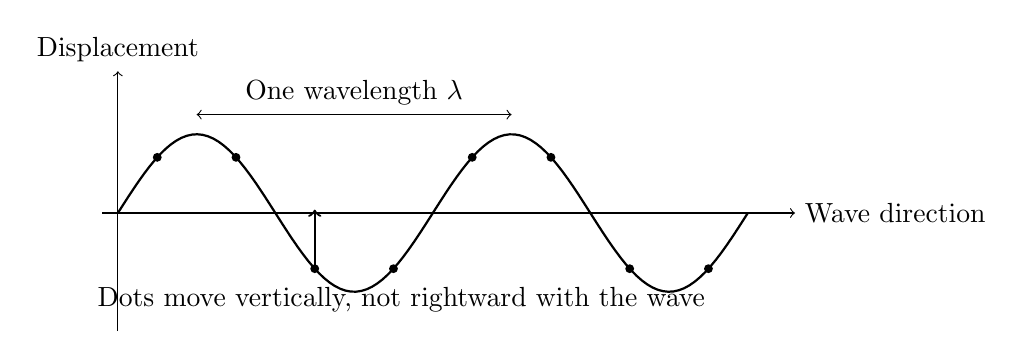
\begin{tikzpicture}[scale=1]
  \draw[->] (-0.2,0) -- (8.6,0) node[right] {Wave direction};
  \draw[->] (0,-1.5) -- (0,1.8) node[above] {Displacement};
  \draw[thick,domain=0:8,samples=120] plot (\x,{sin(\x*90)});
  \foreach \p in {0.5,1.5,2.5,3.5,4.5,5.5,6.5,7.5}
    \fill (\p,{sin(\p*90)}) circle (1.6pt);
  \draw[<->] (1,1.25) -- (5,1.25) node[midway,above] {One wavelength $\lambda$};
  \draw[->,thick] (2.5,{sin(2.5*90)}) -- (2.5,{sin(2.5*90)+0.75});
  \node at (3.6,-1.1) {Dots move vertically, not rightward with the wave};
\end{tikzpicture}
\caption{A transverse wave: the profile travels right while each oscillator, a black dot, moves only up and down locally.}
\end{figure}

\begin{figure}[htbp]
\centering
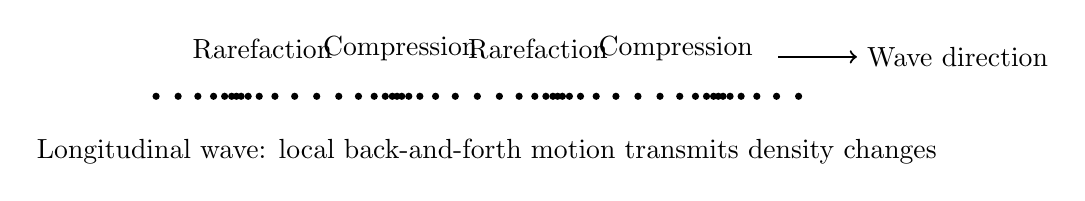
\begin{tikzpicture}[scale=1]
  \foreach \i in {0,...,48}
    \fill ({0.17*\i + 0.22*sin(\i*30)},0) circle (1.3pt);
  \node at (1.35,0.6) {Rarefaction};
  \node at (3.1,0.6) {Compression};
  \node at (4.85,0.6) {Rarefaction};
  \node at (6.6,0.6) {Compression};
  \draw[->,thick] (7.9,0.5) -- (8.9,0.5) node[right] {Wave direction};
  \node at (4.2,-0.7) {Longitudinal wave: local back-and-forth motion transmits density changes};
\end{tikzpicture}
\caption{A longitudinal wave: each point stays near home while rarefaction and compression propagate.}
\end{figure}

\step{The Model in One Sentence}

\begin{oneline}
A wave is a relay among coupled oscillators: each oscillates locally, passing displacement from equilibrium and energy to the next; the message travels, not the matter.
\end{oneline}

\begin{mainline}
Every phrase matters. Coupling explains why the second oscillator moves. Local motion explains why matter does not travel far. Passing to the next explains a definite wave speed, set by each relay's transfer rate and therefore by the medium. Keep message on account; next chapter's sound and information will repay it with interest. Remember the sentence: every later formula merely annotates it.
\end{mainline}

\step{The Mathematical Translator}

\begin{mainline}
Translate intuition into numbers and pictures, beginning with three practical quantities.

\textbf{Period and frequency} come from Chapter 16. Each oscillator's cycle takes period \(T\); cycles per second give frequency \(f=1/T\), in hertz. Every oscillator follows the source's rate: frequency is the source's signature.

\textbf{Wavelength} asks a spatial question. In an instantaneous snapshot, neighboring crests are separated by \(\lambda\).

\textbf{Wave speed} \(v\) measures propagation. A simple relation ties these quantities together. In one source cycle of duration \(T\), a complete new bump forms while the leading bump travels \(vT\). The new and preceding crests are therefore \(vT\) apart, exactly one wavelength:

\[
  \lambda = vT, \qquad \text{or} \qquad v = f\lambda .
\]

What does this describe? The tradeoff between frequency and wavelength for one wave. Why this form? One cycle makes one crest, and speed fixes crest spacing. When does it hold? When \(v\) is uniform throughout the medium, as on a uniform rope or in still uniform air. When does it fail? If speed varies with location or frequency, as for varying water depth or light through glass, \(v\) is no longer constant and each frequency must be handled separately.

Check extremes. Double frequency and wavelength halves: faster source motion crowds crests together. In a medium with speed approaching zero, no frequency propagates and wavelength collapses to zero, as though the medium freezes. Both are sensible.
\end{mainline}

\begin{mainline}
\textbf{Do not confuse two graphs.} Beginners often trip over two different wave pictures. A \textbf{wave-profile graph} snapshots the whole rope at one instant: horizontal position \(x\), vertical local displacement. It tells where bumps and dips are now. An \textbf{oscillation graph} films one oscillator: horizontal time \(t\), vertical displacement. It tells when that point rises and falls. Crest spacing is wavelength in the first, period in the second, spatial and temporal rulers linked by wave speed. A useful skill: given a profile and propagation direction, predict a point's next motion by shifting the whole curve slightly that way and checking whether its new height rises or falls. The profile translates while each point slides on its own vertical line, the graphical version of state traveling rather than matter.
\end{mainline}

\begin{mainline}
\textbf{An account for your ears.} Sound travels through air at about \(340\) meters per second, and human hearing spans roughly \(20\) to \(20000\) hertz. Using \(\lambda = v/f\), the lowest audible note has wavelength about \(17\) meters, longer than a classroom, and the highest about \(1.7\) centimeters, smaller than a button. This range explains everyday experience. Bass-drum wavelengths comparable to walls and doorways readily bend around them, so renovation thumps downstairs seem to penetrate everywhere. High-pitched clinking keys have centimeter wavelengths and travel more nearly straight past obstacles; hiding behind a pillar noticeably muffles them. Pitch, loudness, and timbre correspond to frequency, amplitude, and waveform, next chapter's topic. For now, remember these have tangible scales convertible through \(v=f\lambda\).
\end{mainline}

\begin{mainline}
\textbf{A realistic estimate.} You measured rope-wave speed; now calculate it. Analyzing transverse tension forces on a small stretched-rope segment, as in the mathematical bridge, gives

\[
  v = \sqrt{\frac{T}{\mu}},
\]

where \(T\) is tension and \(\mu\) mass per length, linear density. A medium-tension steel guitar string has tension about \(70\) newtons and mass about \(5\) grams per meter, or \(\mu = 0.005\) kilograms per meter. Thus

\[
  v = \sqrt{\frac{70}{0.005}} = \sqrt{14000} \approx 118\ \text{m/s}.
\]

This immediately helps. A guitar string is about \(0.65\) meters long. Standing waves will show that its fundamental fits half a wavelength between fixed ends, so \(\lambda = 2\times 0.65 = 1.3\) meters. Its fundamental frequency is

\[
  f = \frac{v}{\lambda} = \frac{118}{1.3} \approx 91\ \text{Hz},
\]

close to a real fifth string's open 110-hertz note, differing only by our choice of a somewhat loose string. One string, one formula, and an order-of-magnitude match in pitch: concrete evidence that the medium sets wave speed.
\end{mainline}

\begin{mathbridge}
How do we analyze that rope segment? Displacement \(y\) depends on both position \(x\) and time \(t\), giving \(y(x,t)\). For a small segment, the slightly different tension directions at its ends provide restoring net force. Its mass is \(\mu\,\mathrm{d}x\), and acceleration is the second time derivative of \(y\). Apply Newton's second law and the small-amplitude approximation, meaning small profile slopes everywhere, then cancel \(\mathrm{d}x\):

\[
  \frac{\partial^2 y}{\partial t^2} = \frac{T}{\mu}\,\frac{\partial^2 y}{\partial x^2}.
\]

This is the one-dimensional wave equation. The left is local time acceleration; the right is local spatial curvature times a medium-dependent constant. In words: \textbf{greater local bending gives greater oscillator acceleration back toward equilibrium}. Linking time change to spatial curvature mathematically expresses propagating oscillation. Verify the solution \(y(x,t)=A\sin(kx-\omega t)\), provided \(\omega/k=\sqrt{T/\mu}=v\): \(v=f\lambda\) dressed as a sine wave. Here \(k=2\pi/\lambda\) is wavenumber and \(\omega=2\pi f\) angular frequency. Small-amplitude approximation fails when slopes cease to be small, as in curling huge waves or a string plucked into a sharp corner. More complicated terms must then be added on the right, a limit revisited below.
\end{mathbridge}

\begin{mainline}
\textbf{Two waves meet: our most important counterintuitive fact.} Return to prediction 3. When two bumps approach, displacements simply add where they overlap. The rope's instantaneous position is the sum of where each wave alone would put it. Then the waves pass through each other unchanged in shape and speed, as though nothing happened. They do not bounce apart like billiard balls.

This is \textbf{superposition}: when several waves share a medium, each oscillator's actual displacement is the sum of their separate contributions. It follows directly from the wave equation, containing \(y\) but no squared or cubed \(y\), so a sum of solutions is another solution.

Your ears supply familiar evidence. Two people speaking in one room produce waves that pass through each other, yet both remain intelligible. If sound collided like traffic, it would become chaos. Ears and microphones nevertheless receive only the combined vibration; separating voices afterward is the brain's or algorithm's work. Independent propagation is one of the sharpest differences between waves and particles.

Superposition bears three fruits:

\begin{itemize}
  \item \textbf{Interference}: two equal-frequency sources, such as fingers tapping water together, produce overlapping ripples. At some locations, crests repeatedly meet and motion is strong; elsewhere crest meets trough and water barely moves. This pattern depends only on the path-length difference from the two sources.
  \item \textbf{Reflection and refraction}: at the table leg, a bump cannot proceed and its energy turns back: reflection. A fixed end also inverts it, returning an upward bump downward. Crossing into a different-speed medium, such as deep-to-shallow water, reduces speed while frequency stays fixed. By \(v=f\lambda\), wavelength shortens and propagation direction bends: refraction. Waves reach beaches roughly parallel to shore because slower shallow-water motion turns their fronts shoreward.
  \item \textbf{Diffraction}: an obstacle or aperture does not produce only a straight-edged geometric shadow. Waves spread around its sides. Smaller gaps, especially comparable to wavelength, give stronger spreading. Hearing speech outside a doorway largely relies on sound bending around the frame. Low, long-wavelength components turn corners more readily than short-wavelength high ones, making speech through walls sound muffled.
\end{itemize}
\end{mainline}

\begin{mainline}
\textbf{Standing waves: waves confined by boundaries.} On a string fixed at both ends, rightward waves reflect leftward. Opposite waves of equal frequency usually combine into disorderly motion, but particular frequencies fit an integer number of half-wavelengths exactly into the length. Their sum has a stable shape oscillating in place, with permanently still nodes and maximally moving antinodes. These are the standing waves you found in Step 2. Allowed frequencies are

\[
  f_n = n\,\frac{v}{2L}, \qquad n=1,2,3,\dots
\]

where \(L\) is string length. These discrete \textbf{eigenfrequencies} are its identification numbers. Guitars, violins, and pianos use them for pitch: bridge and nut fix \(L\), while tuning changes tension \(T\), hence \(v\). Wind instruments retell the same story with air columns, longitudinal oscillator chains, whose length replaces string length. Fingering changes effective air-column length and its eigenfrequencies. Test it in the kitchen: blowing across a bottle gives a low note; add water and it rises. Higher water shortens the air column, reducing \(L\), and \(f_n = nv/(2L)\) raises frequency. Why does a table give a thud while a string sings? A table's complex shape crowds allowed frequencies into irregular ratios, while a string's frequencies line up as \(1:2:3:\cdots\), an order the ear hears as pitch.
\end{mainline}

\begin{figure}[htbp]
\centering
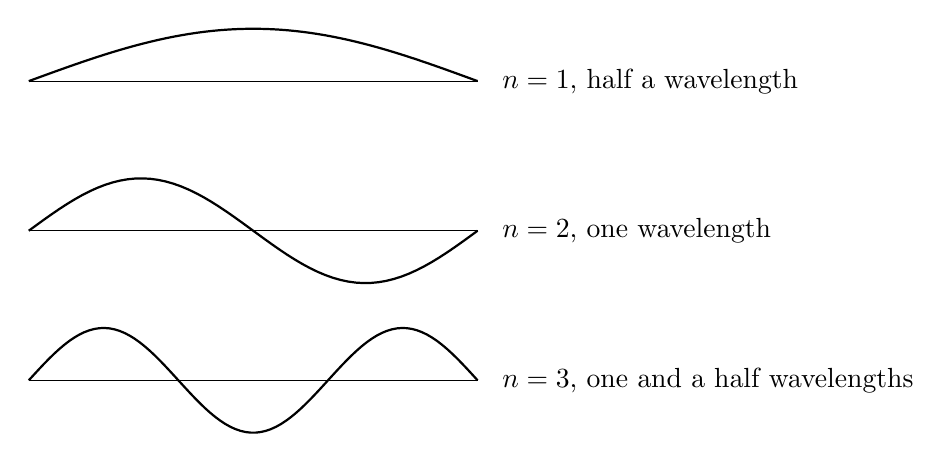
\begin{tikzpicture}[scale=0.95]
  \begin{scope}
    \draw (0,0) -- (6,0);
    \draw[thick,domain=0:6,samples=60] plot (\x,{0.7*sin(\x*30)});
    \node[right] at (6.2,0) {$n=1$, half a wavelength};
  \end{scope}
  \begin{scope}[yshift=-2cm]
    \draw (0,0) -- (6,0);
    \draw[thick,domain=0:6,samples=60] plot (\x,{0.7*sin(\x*60)});
    \node[right] at (6.2,0) {$n=2$, one wavelength};
  \end{scope}
  \begin{scope}[yshift=-4cm]
    \draw (0,0) -- (6,0);
    \draw[thick,domain=0:6,samples=90] plot (\x,{0.7*sin(\x*90)});
    \node[right] at (6.2,0) {$n=3$, one and a half wavelengths};
  \end{scope}
\end{tikzpicture}
\caption{Three standing waves allowed on a fixed-end string. Only integer numbers of half-wavelengths fit its length exactly.}
\end{figure}

\step{The Model's Limits}

\begin{mainline}
An honest model states where its work ends.

\textbf{Boundary 1: a medium is required; these are mechanical waves.} Rope, water, air, and ground waves all relay among material oscillators. Without matter, there is no relay. This is a definition, not a defect, but immediately raises a question: what relays sunlight through vacuum? The electromagnetic section will answer. Electric and magnetic fields are physical properties of space whose changes propagate together under Maxwell's equations, needing no material medium. You will appreciate learning the abstraction of propagating state here; electromagnetic waves transfer it from matter to fields.

\textbf{Boundary 2: small amplitude and linearity.} Superposition, \(v=f\lambda\), and the wave equation assume small displacements and proportional restoring force. High waves curl and break; powerful sound compresses into shocks, sonic booms. Wave speed then depends on amplitude, strong waves overtake and swallow weaker ones, superposition fails, and profiles change during propagation. Speech, musical strings, and pond ripples lie inside the safe region; explosions, sonic booms, and breaking surf lie outside.

\textbf{Boundary 3: a uniform stationary medium and stationary source.} Wind or water flow adds medium motion to apparent wave speed. Nonuniform media, such as ocean temperature layers or warm air below cold, make speed vary continuously and bend waves. Above hot ground on summer afternoons, sound bends upward and travels poorly; cool near-ground night air bends it back, helping distant trains be heard for reasons beyond quiet surroundings. A moving source gives another departure: an approaching ambulance sounds higher, a receding one lower, not because sound speed changes but because the source crowds wavefronts ahead and stretches them behind. This Doppler effect formally belongs to next chapter, but its foundation is here. Wavelength changes, but in \(v=f\lambda\), the speed \(v\) remains air's decision.

\textbf{Typical misuses}: first, waves transport the objects themselves. No: states and energy travel, while floats and spectators remain local. Second, the medium sets frequency. No: the source sets frequency, the medium sets speed, and wavelength follows from both. Third, standing waves are two stopped waves. No: both still pass through each other at their original speed; only their combined profile stands still.
\end{mainline}

\begin{challenge}
Do all frequencies travel equally fast in one medium? Ideal ropes and air say yes: wave-equation \(v\) contains no frequency. Deep-water waves and light in glass say no, a phenomenon called \textbf{dispersion}. Then distinguish two speeds. \textbf{Phase velocity}, \(v_p=\omega/k\), is the speed of a fixed phase point, such as a crest. \textbf{Group velocity}, \(v_g=\mathrm{d}\omega/\mathrm{d}k\), is the speed of an entire wave packet. Energy and information accompany that packet, so signal speed means group velocity. Watch the edge of ripples after dropping a stone: individual ripples appear inside the packet, cross it, and vanish at its outer edge. Individual waves travel faster than the packet. Their relative speeds depend on the dispersion relation \(\omega(k)\). Quantum matter waves bring them back: phase velocity can exceed light speed but group velocity cannot, because the latter matches particle motion and preserves causality.
\end{challenge}

\step{Explaining the Opening Phenomenon}

\begin{mainline}
Now grade the opening questions.

Why does shouting produce no gale? Sound is a longitudinal relay. Vocal cords push nearby air back and forth; each molecule moves locally less than a hair's width, passing dense--thin--dense states onward. After \(0.3\) seconds the state reaches Xiaoming and moves his eardrum. No air travels across, but the message arrives intact. Your vocal cords set frequency, which lets him recognize your voice; air temperature and elasticity set speed, \(340\) meters per second, and wavelength follows.

Why does the duck merely bob? In ideal water waves, each molecule moves in a small local circle. Motion state and energy propagate, while the duck follows local circular movement as a surface marker, without drifting. Wind or currents genuinely transporting water are a separate matter.

Why does a stadium wave circle the stands? It displays state relay plainly: people stand and sit; your turn propagates. Estimate: a wave circles a roughly four-hundred-meter stadium in twenty-something seconds, at tens of meters per second. Spectators half a meter apart pass the standing state twenty-something times each second, consistent with a person's few-tenths-second reaction to a rising neighbor. Its speed table contains reaction time, not tension or mass: an unusual medium's version of medium-determined speed.

Another application is earthquake early warning. Quakes launch longitudinal P waves at about \(6\) kilometers per second and transverse S waves at about \(3.5\), with S waves far more damaging. Monitoring networks detect faster, gentler P waves, then warn farther cities by electromagnetic signals traveling about 300,000 kilometers per second, effectively instantaneously here, before S waves arrive. Chengdu's warning system has gained urban areas tens of seconds in several earthquakes, allowing trains to slow, surgery to pause, and elevators to reach nearby floors. Those seconds come from one core fact: \textbf{media determine wave speeds, and those speeds differ enormously}.
\end{mainline}

\step{Thought Experiments and Challenges}

\begin{thought}[A Steel Cable from Earth to the Moon]
Imagine a taut steel cable between Earth and Moon, ignoring how many pieces its own weight would break it into. Strike Earth's end with a hammer. When can someone on the Moon know?

Longitudinal waves travel through steel at about \(5000\) meters per second. Across roughly \(38\) ten-thousand kilometers, the compression relay takes \(380000000/5000 = 76000\) seconds, about \(21\) hours. Radio takes only \(1.3\) seconds over the same route, nearly sixty thousand times faster than this mechanical signal.

An astronaut touching an ear to the cable could hear it, while one floating beside it could not. Vacuum has no air-oscillator chain to relay sound. Thunderous space explosions in science fiction belong to directors, not physics.
\end{thought}

\begin{mainline}
Connect this chapter to the book's map. Neighbor coupling takes us from one oscillator in Chapter 16 to many here. The recipe is powerful and repeatedly reusable. Replace oscillators with a row of charges and coupling with electric and magnetic fields to approach electromagnetic waves. Remember strings' discrete eigenfrequencies: atomic electrons likewise occupy a discrete set of standing-wave-like states. Fitting integer half-wavelengths into finite space supplied early intuition for energy quantization. Modern field theory even treats every spatial point as an oscillator and particles as quanta of field vibration. One oscillator vibrates; many make a wave. The rest of that sentence waits in the quantum section.
\end{mainline}

\begin{puzzles}
  \item An astronaut taps a space-station wall. A crewmate inside hears it, but a spacewalker outside, without a helmet pressed against it, does not. Identify each relay chain and its missing link. (Hint: inside, one chain is metal wall plus cabin air. What is absent outside?)
  \item Tightening a guitar string raises pitch. Use our formulas to write every step from turning the peg to hearing a higher note, without numbers. (Hint: which quantity does the peg change? Does it first affect \(v\) or \(f\)? Has length changed?)
  \item Shout at a distant cliff and hear an echo. Saying sound collides with the cliff and bounces back is half right: reflection reverses energy flow, but collision hides boundary conditions. A rope's fixed-end reflection inverts crest into trough. Does sound reflected by a hard cliff invert? (Hint: can the air move freely at the cliff? Is that more like a rope's fixed or free end?)
  \item What sets a stadium wave's speed? Compared with rope-wave factors, what resembles elasticity and what resembles inertia? Would spectators reacting twice as fast make it faster, and what rope change would that resemble? (Hint: there is no physical restoring force; the relay follows an observation--reaction chain. How far can the analogy about speed-setting mechanisms go?)
\end{puzzles}
